\documentclass[notoc]{JHEP3}
\usepackage{cite,color,psfrag,url,latexsym,graphicx,epstopdf,slashed,xspace,hyperref,enumitem,lineno}
\let\normalcolor\relax

\newcommand{\event}{ {\sc event2}}
\newcommand{\In}{ {\rm in}}
\newcommand{\Out}{ {\rm out}}
\newcommand{\nbar}{ {\bar{n}}}

\newcommand{\ds}{\displaystyle}
\newcommand{\Ord}{\mathcal{O}}
\newcommand{\sL}{\mathcal{L}}
\newcommand{\nn}{\nonumber \\}
\newcommand{\el}{\nonumber \\ &&}
\newcommand{\ezint}[3]{\int_{#1}^{#2} d #3}
\newcommand{\mint}[1]{\int {d^d #1 \over (2 \pi)^d}}
\newcommand{\mintd}[2]{\int {d^{#2} #1 \over (2 \pi)^{#2}}}
\newcommand{\mintb}[1]{\int d^d #1}
\newcommand{\M}{\mathcal{M}}
\newcommand{\T}{\theta}
\newcommand{\pt}{$p_{T}$}
\newcommand{\eqref}[1]{(\ref{#1})}
\newcommand{\text}[1]{{\rm #1}}
\newcommand{\jw}{\textsc{Jewel}~}
\newcommand{\jwpy}{\textsc{Jewel+Pythia}~}
\newcommand{\py}{\textsc{Pythia}~}
\newcommand{\bS}{\hat{S}}
\newcommand{\rS}{S_r}
\newcommand{\GNGL}{\Gamma^{\mathrm{NGL}}}
\newcommand{\gsreg}{\gamma^{\mathrm{NGL}}}

\newcommand{\thR}{R}
\newenvironment{changemargin}[2]{%
  \begin{list}{}{%
    \setlength{\topsep}{0pt}%
    \setlength{\leftmargin}{#1}%
    \setlength{\rightmargin}{#2}%
    \setlength{\listparindent}{\parindent}%
    \setlength{\itemindent}{\parindent}%
    \setlength{\parsep}{\parskip}%
  }%
  \item[]}{\end{list}}

\def\PlusBreak#1{+ \nonumber \\          % splits line with plus sign
          &&  \hphantom{#1} \! \null   +}
\def\MinusBreak#1{- \nonumber \\         % splits line with minus sign
          &&  \hphantom{#1} \!  \null  -}
\def\TimesBreak#1{\times \nonumber \\    % splits lines with times sign
          &&  \hphantom{#1} \!  \null  \times}


% The following macros allow line splits allowing for line spacing adjustments
% 12 is line spacing e.g. 1pt plus 4pt and #2 is the hphantom
\def\PlusBreakAdjust#1#2{+ \nonumber \\ [#1]      % splits line with plus sign
          &&  \hphantom{#2} \! \null  +}
\def\MinusBreakAdjust#1#2{- \nonumber \\ [#1]     % splits line with minus sign
          &&  \hphantom{#2} \!  \null -}
\def\TimesBreakAdjust#1#2{\times \nonumber \\[#1] %splits lines with times sign
          &&  \hphantom{#2} \!  \null  \times}

\def\eqn#1{Eq.~(\ref{eq:#1})}
\def\Eqn#1{Eq.~(\ref{eq:#1})}
\def\eqns#1#2{Eqs.~(\ref{eq:#1}) and~(\ref{eq:#2})}
\def\Eqns#1#2{Eqs.~(\ref{eq:#1}) and~(\ref{eq:#2})}
\def\fig#1{Figure~{\ref{fig:#1}}}
%\renewcommand{\sec}[1]{Section~\ref{sec:#1}}
\newcommand{\ssec}[1]{Section~\ref{ssec:#1}}
\newcommand{\be}{\begin{equation}}
\newcommand{\ee}{\end{equation}}
\newcommand{\cmb}{\begin{changemargin}}
\newcommand{\cme}{\end{changemargin}}
\newcommand{\bea}{\begin{eqnarray}}
\newcommand{\eea}{\end{eqnarray}}
% \newcommand{\bea}{\begin{align}}
% \newcommand{\eea}{\end{align}}

\newcommand{\highlightA}{black}
\newcommand{\highlight}{black}

\newcommand{\D}{\delta}
\newcommand{\g}{\gamma}
\newcommand{\A}{\alpha}
\newcommand{\B}{\beta}
\newcommand{\G}{\Gamma}
\newcommand{\la}{\leftarrow}
\newcommand{\ra}{\rightarrow}
\newcommand{\mc}{\mathcal}
\newcommand{\mb}{\mathbb}
\newcommand{\gcusp}{\Gamma_{\rm cusp}}
\newcommand{\rr}{\frac{R}{1-R}}
\newcommand{\lib}{{\mathrm{Li}_2}}
\newcommand{\lic}{{\mathrm{Li}_3}}
\newcommand{\tauo}{\tau_\omega}
\newcommand{\bn}{{\bar{n}}}
\newcommand{\ecm}{E_{\rm CM}}
\newcommand{\dd}{\mathrm{d}}
\newcommand{\als}{\alpha_s}
\newcommand{\ep}{\epsilon}
\newcommand{\ws}{\widetilde{s}}
\def\Tr{\mathop{\rm Tr}\nolimits}
\def\TrFf{\mathop{\rm Tr}\nolimits F^4}
\def\si{\sigma}
%\newcommand{\SU}{\mathop{\rm SU}\nolimits}
\def\spa#1.#2{\langle#1\,#2\rangle}
\def\spb#1.#2{[#1\,#2]}
\def\sandmm#1.#2.#3{%
\left\langle\smash{#1}{\rphantom1}\right|{#2}%
\left|\smash{#3}{\rphantom1}\right]}
\def\spab#1.#2.#3{\sandmm#1.#2.#3}
\def\spba#1.#2.#3{\sandpp#1.#2.#3}
\def\spaa#1.#2.#3.#4{\sandmp#1.{#2#3}.#4}
\def\spbb#1.#2.#3.#4{\sandpm#1.{#2#3}.#4}
\def\spash#1.#2{\spa{\smash{#1}}.{\smash{#2}}}
\def\spbsh#1.#2{\spb{\smash{#1}}.{\smash{#2}}}

\def\ksl{\not{\hbox{\kern-2.3pt $k$}}}
\def\lsim{\lesssim}
\def\gsim{\gtrsim}
\def\susy{{\rm susy}}
\def\ib{{\bar\imath}}
\def\cg{c_\Gamma}
\def\e{\epsilon}
\def\musq{\mu^2}
\def\tree{{\rm tree}}
\def\oneloop{{\rm 1\! -\! loop}}
\def\twoloop{{\rm 2\! -\! loop}}
\def\Ord{{\cal O}}
\def\a{{\cal A}}
\def\cm{{\cal M}}
\def\Ft{\tilde{F}}
\def\Re{{\rm Re}}
\def\Nc{N_c}
\def\Nsym{{\cal N}=4}
\def\la{\langle}
\def\ra{\rangle}
\def\bom#1{{\mbox{\boldmath $#1$}}}
%
%
\def\lr{\leftrightarrow}
\def\li#1{{\mathop{\rm Li}\nolimits}_#1}
\def\Li{\mathop{\rm Li}\nolimits}
\def\ggtogg{{gg \to gg}}
\def\alphas{\alpha_s}
\def\draftnote#1{{\it #1}}

\def\rg{r_\Gamma}
\def\Triint{{\rm Tri}}
\def\Boxfour{{\rm Box}^{(4)}}
\def\Boxsix{{\rm Box}^{(6)}}
\def\Boxeight{{\rm Box}^{(8)}}

\def\I{{\cal I}}
\def\pol{\varepsilon}

\def\in{{\rm in}}
\def\out{{\rm out}}
\def\tom{\tau_\omega}
\newcommand{\rd}{\mathrm{d}}

\newcommand{\note}[1]{\marginpar{\footnotesize\textbf{NOTE}} (\textbf{\textcolor{blue}{#1}})}
\newcommand{\todo}[1]{\marginpar{\textbf{\textcolor{blue}{TODO}} \footnotesize{#1}} (\textbf{\textcolor{blue}{TODO}})}

\DeclareRobustCommand{\Sec}[1]{Sec.~\ref{#1}}
\DeclareRobustCommand{\Secs}[2]{Secs.~\ref{#1} and \ref{#2}}
\DeclareRobustCommand{\Secss}[3]{Secs.~\ref{#1}, \ref{#2} and \ref{#3}}
\DeclareRobustCommand{\App}[1]{App.~\ref{#1}}
\DeclareRobustCommand{\Tab}[1]{Table~\ref{#1}}
\DeclareRobustCommand{\Tabs}[2]{Tables~\ref{#1} and \ref{#2}}
\DeclareRobustCommand{\Fig}[1]{Fig.~\ref{#1}}
\DeclareRobustCommand{\Figs}[2]{Figs.~\ref{#1} and \ref{#2}}
\DeclareRobustCommand{\Figss}[3]{Figs.~\ref{#1}, \ref{#2} and \ref{#3}}
\DeclareRobustCommand{\Eq}[1]{Eq.~(\ref{#1})}
\DeclareRobustCommand{\Eqs}[2]{Eqs.~(\ref{#1}) and (\ref{#2})}
\DeclareRobustCommand{\Eqss}[3]{Eqs.~(\ref{#1}), (\ref{#2}), and (\ref{#3})}
\DeclareRobustCommand{\Ref}[1]{Ref.~\cite{#1}}
\DeclareRobustCommand{\Refs}[2]{Refs.~\cite{#1} and \cite{#2}}

\title{Probing heavy ion collisions using quark and gluon jet substructure with machine learning}

\author{Yang-Ting Chien $^{a}$ and Raghav Kunnawalkam Elayavalli $^{b}$\\
$^{a}$ Center for Theoretical Physics\\
$~$ Massachusetts Institute of Technology, Cambridge, MA 02139, USA\\
$^{b}$ Department of Physics and Astronomy\\
$~$ Rutgers, the State University of New Jersey, New Brunswick, NJ 08901, USA\\
}

\abstract{
We study the classification of quark-initiated jets and gluon-initiated jets in proton-proton and heavy ion collisions using modern machine learning techniques. We train the deep convolutional neutral network on discretized jet images. The classification performance is compared with the multivariate analysis of several physically-constructed jet observables including the jet mass, the $p_T^D$, the multiplicity and the radial moments. We also compare with the systematic $N$ subjet expansion in telescoping deconstruction to exploit the information carried by the subjets. The quark and gluon jet samples generated from \jw are used as an example to demonstrate this general method. We find that the classification performance goes down in the \textsc{Jewel}-simulated heavy ion collisions. The information carried by the subleading subjets can be washed out by the possible subjet thermalization or randomization due to the soft event activities. Our method provides a systematically improvable framework for analyzing and comparing all jet simulations and measurements in heavy ion collisions.
}

\begin{document}

\section{Introduction}
\label{sec:intro}

The jet quenching phenomenon observed at the Relativistic Heavy Ion Collider (RHIC) \cite{Adcox:2001jp,Adler:2002xw,Adcox:2004mh,Arsene:2004fa,Back:2004je,Adams:2005dq}
and the Large Hadron Collider (LHC)\cite{Aamodt:2010jd,Abelev:2012hxa,Abelev:2013kqa,Aad:2012vca,Aad:2014bxa,Chatrchyan:2013kwa,
Chatrchyan:2012gw,Chatrchyan:2014ava,Aad:2014wha,Chatrchyan:2013exa,
Adam:2015ewa,Chatrchyan:2012gt,Chatrchyan:2011sx,Chatrchyan:2012nia,Aad:2010bu,Aad:2013sla,Adam:2015doa,Aad:2015bsa} has since become an essential hard probe of the strongly interacting medium produced in heavy ion collisions. Traditionally jet quenching refers to the dramatic suppression of hadron and jet cross sections, which is translated into the parton and jet energy loss picture. It is now established that the lost energy distributes within an angle of $O(1)$ from the jet through the missing transverse momentum measurement. By studying in details how the jet energy redistributes in heavy ion collisions, one can quantitatively extract the information about the jet-medium interaction and the underlying medium dynamics. The heavy ion jet physics has thus moved to the era of precision jet substructure and classified jet cross section studies.

The jet substructure measurements provide concrete information about the modifications of jets. From the measurements of the jet shape and jet fragmentation function, we have learned that both the transverse and longitudinal momentum distributions inside jets are significantly modified. Since jet substructures depend strongly on the partonic origin of jets, the change of the fraction of quark-initiated jets and gluon-initiated jets will contribute to the substructure modifications. It has been realized that the increase of the quark jet fraction in heavy ion collisions constitutes the narrowing of the jet cores seen in various inclusive jet substructure measurements. With purer quark and gluon jet samples, one can disentangle the effect from the changing quark and gluon jet fractions and focus on the jet-by-jet modifications. Quark jets and gluon jets can then be used as independent probes.

We will study the tagging of quark and gluon jets making full use of their substructure information. In contrast to the conventional wisdom of directly comparing jets in proton-proton and heavy ion collisions, this indirect approach studies the modification of the comparison between different probes. By first comparing the probes in the same system, it may help reducing the systematic uncertainty in experimental measurements. The lowest order feature which separates quark jets from gluon jets is the different color charges carried by the jet-initiating partons. The Casimir factors of quark jets and gluon jets are $C_F = 4/3$ and $C_A=3$ respectively, and the larger color charge of gluons results in the broader spread of the radiations inside gluon jets. Various jet substructure variables have been used and combined to further increase the tagging performance with a multivariate analysis, and the advances of machine learning techniques have been constantly incorporated in solving this classification problem.

In this paper we benchmark three classes of methods in quark and gluon tagging and gain insights from comparing their performances. We use modern image recognition techniques utilizing deep convolutional neural networks (DCNN). The network is trained on the discretized images of quark jets and gluon jets, and the samples are generated from the \jw heavy ion event generator. Different simulations may produce differently characteristic quark and gluon jets, and this method can help compare simulations and be extended to using the data from experiments. We also examine the tagging performance using five physically constructed jet substructure variables: the jet mass, the $p_T^D$, the multiplicity and two radial moments including the girth. Subsets of the variables are combined and studied in a multivariate analysis using boosted decision trees, and we look into the correlations among the variables. Lastly, we systematically expand the information within jets using the recently developed telescoping deconstruction method. The corresponding subjet expansion can be truncated at any finite order $N$ which allows us to access the information carried by the subleading subjets.

The rest of the paper is organized as follows. In Sec.~\ref{sec:sample} we describe the jet samples we generate using the \jw simulation. In Sec.~\ref{sec:tagger} we give the details about the jet image, the multivariate analysis and the telescoping deconstruction methods. In Sec.~\ref{sec:results} we show the performance of each method and the distributions of jet substructure observables. In Sec.~\ref{sec:conc} we conclude and give an outlook of future studies.

\section{Jet Samples}
\label{sec:sample}

We use the \textsc{Jewel} simulation to generate the quark-initiated and gluon-initiated jet samples through the prompt photon production channels \cite{}. The quark jets are generated by $pp\rightarrow q +\gamma$ in proton-proton collisions and ${\rm PbPb}\rightarrow q+\gamma$ in central (0-20\%) lead-lead collisions at at $\sqrt{s} = 2.76$ TeV using the standard \jw setup \cite{Zapp:2013zya}. Similarly gluon jets are generated by the $g +\gamma$ channel.

\jw is a perturbative QCD Monte Carlo framework for simulating jets in proton-proton and heavy ion collisions. The medium-induced energy loss in heavy ion collisions is based on a simple medium model consisting of thermal scattering centers undergoing the Bjorken expansion. We set the medium formation time $\tau_\text{i}=0.6 $ fm and initial temperature $T_\text{i}=485$ MeV from the hydrodynamic calculation~\cite{Shen:2012vn,Shen:2014vra}. We use the \textsc{Cteq6LL} \cite{Pumplin:2002vw} and \textsc{Eps09}~\cite{Eskola:2009uj} parton distribution functions in \textsc{Lhapdf}~\cite{Whalley:2005nh}.




%For a detailed description of the MC implementation of the jet production and its elastic/inelastic interactions with the scattering centers along with the LPM effect in \jw, please refer~\cite{}. The medium formation time and initial temperature are $\tau_\text{i}=0.6 $fm and  $T_\text{i}=485$ MeV are taken from a hydrodynamic calculation~\cite{Shen:2012vn,Shen:2014vra}. The PDF sets for pp and PbPb sample are \textsc{Cteq6LL}~\cite{Pumplin:2002vw} and \textsc{Eps09}~\cite{Eskola:2009uj} provided by \textsc{Lhapdf}~\cite{Whalley:2005nh}.The primary event collection was split into two halves, with one utilized for training the model(s) and the other for testing \textcolor{red}{additional to a di-jet sample, with a mixture of quark and gluon jets utilized for further evaluation of the model performance}.
	Jets are clustered with the anti-k$_{t}$ algorithm~\cite{} with the distance parameter $R = 0.4$ available in \textsc{fastjet}~\cite{} and the \jw HepMC files~\cite{} are analyzed using the \textsc{Rivet} analysis framework~\cite{}.

The question of what constitutes a "quark" or "gluon" jet is a topic of current discussion~\cite{} but for this paper, we choose the conventional definition of a quark/gluon jet with its progenitor hard scattered parton.

The kinematic cuts for jets in the analysis are $p^{\gamma}_{T} > 100, p^{jet}_{T} > 50$ GeV/c, $|\eta| < 2.0$ and $\Delta \phi_{\gamma, jet} > 2\pi/3$ to ensure that we are selecting the jet that recoils against the isolated $\gamma$.

	There are two operational modes of generating \jw events in heavy ion collisions; with and without including the recoil partons, those originating from interactions of the propagating hard scattered parton with the scattering centers. In recent studies, \jw with recoils was shown to accurately reproduce several of the important qualitative features in jet structure modifications measured by LHC experiments with the addition of background subtraction techniques introduced here~\cite{}. The jet-background in \jw consists of the scattering center's thermal momenta i.e, their momentum before the interaction. For our analysis, we compare the performance of the quark-gluon tagging for three different collections of \jw jets generated with recoils
	\begin{itemize}
		\item no grid and no background subtraction
		\item events discretized in a $\eta-\phi$ grid (0.08 x 0.08) and no background subtraction
		\item discretized events with GridSub background subtraction technique.
	\end{itemize}
	In studying these different jet collections, we extract the dependence of the tagging on key operations performed on jets in data, primarily discretization and background subtraction and discuss their impact on the physics.

\section{Taggers}
\label{sec:tagger}

	Introduce the different taggers in these collisions and talk about how one can study these.

\subsection{Multivariate Analysis}
\label{sec:mva}

	Multivariate analysis have recently been successfully employed in object classification and selection by the LHC experiments and thus are an effective physics driven baseline for our model comparisons. We choose the following five jet observables that highlight differences in the fragmentation patterns for quark and gluon jets as input to our model
	\begin{itemize}
		\item Number of jet constituents, including charged and neutral; given by the anti-k$_{t}$ algorithm
		\item Invariant Jet Mass - utilizing the 4-vector sum of the jet constituents  $M = \sqrt{E^{2} - p^{2}}$
		\item $p_{T}^{D}$ - motivated by the jet fragmentation $p^{D}_{T} = \frac{\sqrt{\sum_{i \in jet} p^{2}_{T,i}}}{p_{T, jet}}$
		\item 0.5 Radial moment - $\sum_{i \in jet} \frac{p_{T, i} (\Delta R_{jet, i})^{0.5}}{p_{T, jet}}$
		\item 1st radial moment (girth) - $\sum_{i \in jet} \frac{p_{T, i} (\Delta R_{jet, i})}{p_{T, jet}}$
	\end{itemize}
	
	 In Fig:~\ref{fig:jetdistributons_pp_pbpb} showcases the distributions of the aforementioned QCD-motivated jet observables in pp and PbPb collisions. The quark and gluon jets shown in Fig:~\ref{fig:jetdistributons_pp_pbpb} include the smearing effect of the grid and in the case of central PbPb, include the GridSub background subtraction method. All five jet observables showcase the ability to classify quarks vs gluons in both pp and PbPb. Recent results from LHC experiments on the effect of jet quenching on inclusive jets showcase two main features; a slight narrowing of the jet core and increased low \pt particle multiplicity in the periphery regions of the jet leading to a broadening of the jet shape. Such an effect is captured in \jw, with the introduction of the medium induced recoils and introduces a further complexity in the question of quark vs gluon classification in PbPb. In vacuum, we expect gluon jets to be broader than quark jets due to the different in the casimir color factor and thus in PbPb collisions, with both jets being quenched and broader, the ability to discriminate effectively between quark and gluon jets is expected to reduce when one only considers fragmentation based observables as we proceed to show in the upcoming sections.
	
	 However, it is important to note that these observables and their distributions in an experiment are highly dependent on the jet clustering algorithm, the minimum \pt cutoff for constituents and the background subtraction procedures employed. In order to facilitate a direct comparing of experiment with MC, one has to either unfold the detector resolution from these observables\footnote{The unfolding procedure for jet observables increases in dimensionality and complexity as the correlations between observables become strong. For example, the invariant jet mass has to be unfolded in 4-D of the generated and reconstructed jet \pt and mass} or run the MC through a simulation of the detector response.
	
	\begin{figure}[h]
	   \centering
	   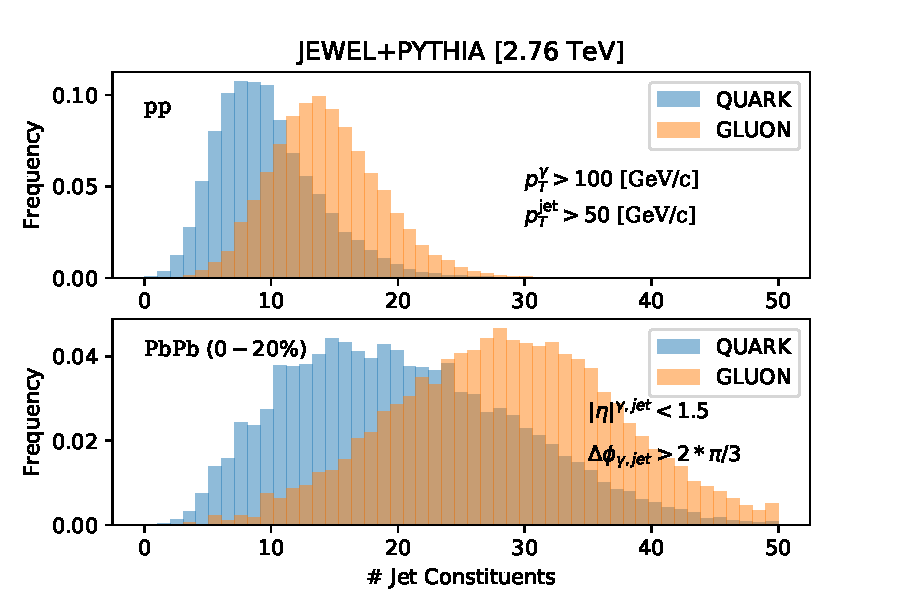
\includegraphics[width=0.45\textwidth]{plots/JEWEL_pp_pbpb020_NumberjetConstituents}
	   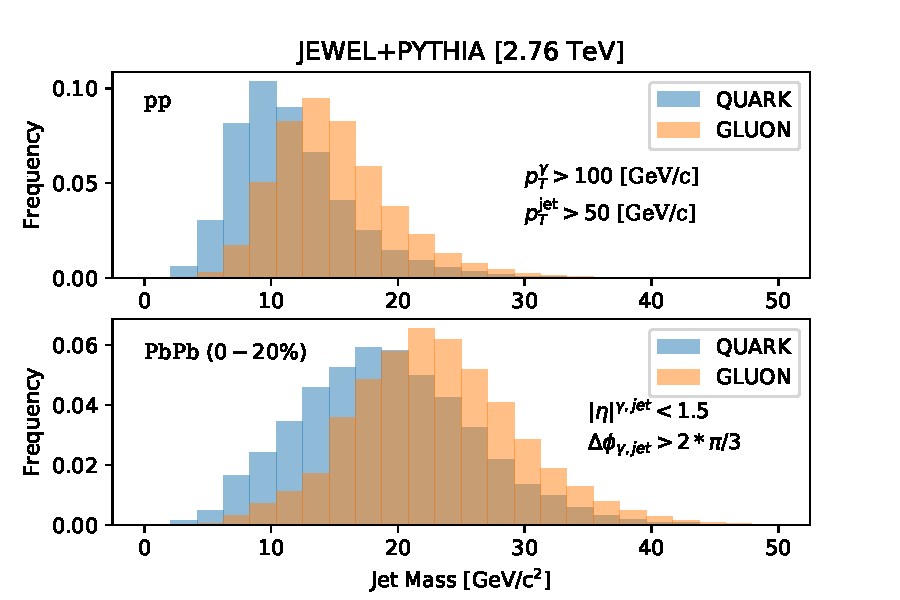
\includegraphics[width=0.45\textwidth]{plots/JEWEL_pp_pbpb020_jetMass}
	   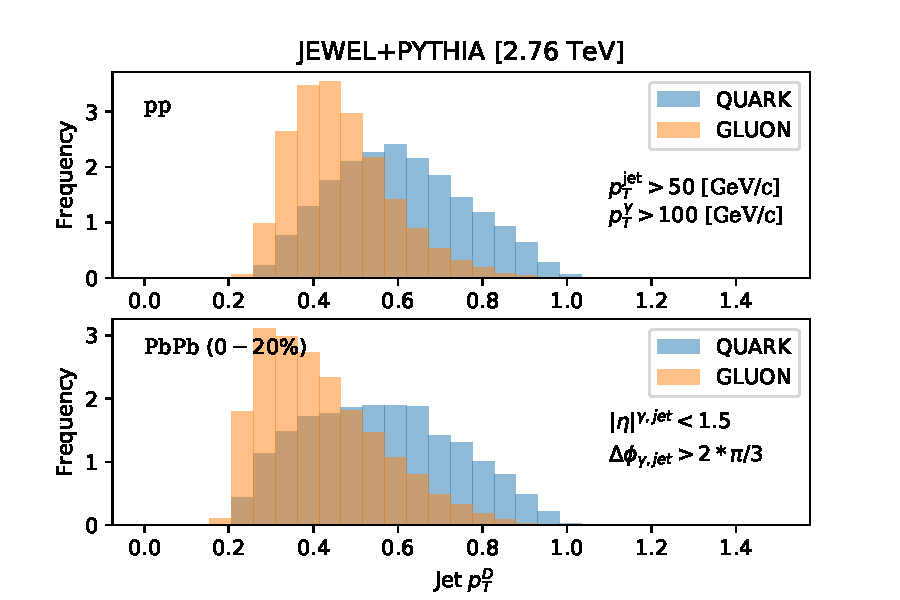
\includegraphics[width=0.45\textwidth]{plots/JEWEL_pp_pbpb020_pTD}
	   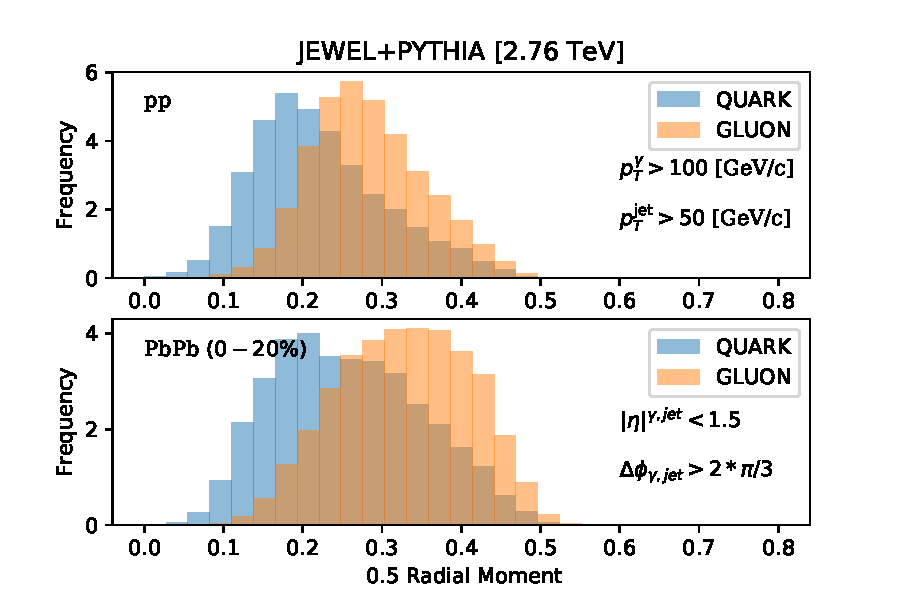
\includegraphics[width=0.45\textwidth]{plots/JEWEL_pp_pbpb020_halfRadialMoment}
	   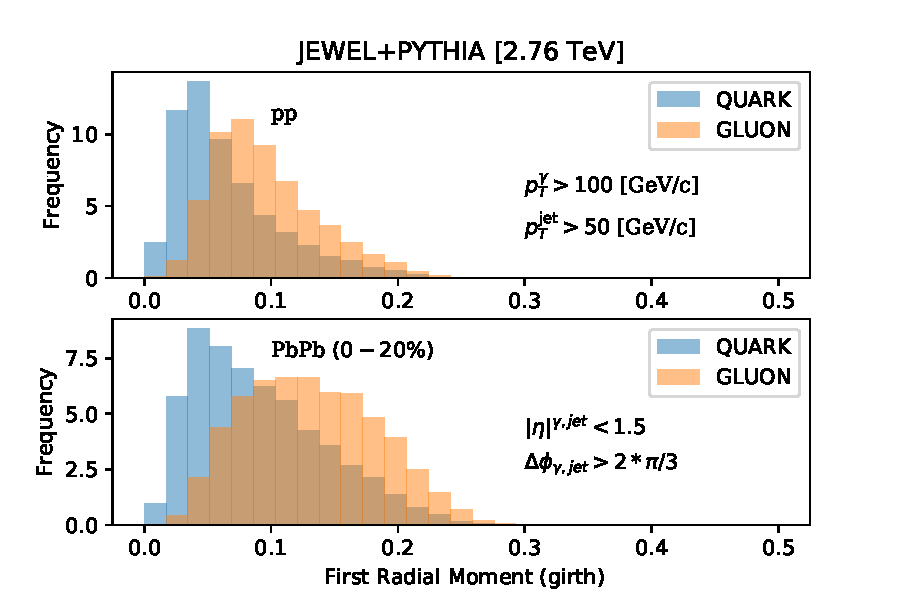
\includegraphics[width=0.45\textwidth]{plots/JEWEL_pp_pbpb020_firstRadialMoment}
	   \caption{Distributions of the jet constituents (top left), invariant jet mass (top right), $p^{D}_{T}$ (center left), the half radial moment (center right) and the jet girth or the first radial moment (bottom) for quark (darker blue) and gluon (lighter orange) induced jets (color online). The top panels of each individual distribution show the pp and the bottom panels correspond to central (0-20\%) PbPb events generated by the \jw generator.}
	   \label{fig:jetdistributons_pp_pbpb}
	\end{figure}
		
	The Multivariate model is defined in Keras with the aforementioned 5 input parameters followed by two dense layers with 10 nodes each. We use the rectified linear (\textit{relu}), and sigmoid activation functions for the dense nodes and the final output layer respectively. The model utilizes the Adam optimizer and it is trained for minimizing binary cross entropy the loss function. We perform cross validation on our MC sample by splitting it into two halves and keeping one for training and the other for testing.


\subsection{Jet Image}
\label{sec:image}

	The radiation pattern of a jet can be visualized as an image in the $\eta-\phi$ plane as seen by a detector with finite segmentation, much like a digital camera~\cite{}. The jet image thus represents a fixed dimensional representation of the energy deposition in the $\eta-\phi$ plane with 'color' of each pixel noted by its \pt. The size of each pixel in a jet image is especially important since. Each jet image follows the pre-processing prescription given in ~\cite{deOliveira:2015xxd} which includes fixing the highest pixel in the jet image as the origin (involving translations in $\eta$ and $\phi$) and rotating the jet image in the plane so that the principal component of the energy density is in the downward direction. This ensures a standard template for the jet image and helps in model performance. Average quark (left) and gluon jet (right) images in pp (top) and central PbPb (bottom) collisions are shown in Fig:~\ref{fig:qgjetimages} where the z axis shows the momentum scale of the jet constituents. As expected, we see a broader energy distribution around the center pixel when they are initiated by gluons in comparison with quarks in pp, whereas both categories of jets are broader in PbPb due to jet quenching effects.  It is important to note the scale of the pixel \pt in the z axis shows jet constituents with experimentally unobservable momenta due to the averaging procedure.

	\begin{figure}[h]
	   \centering
	   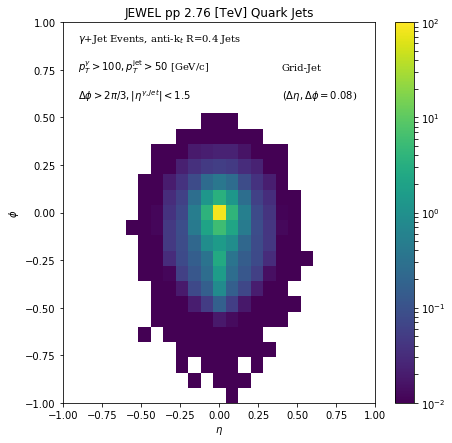
\includegraphics[width=0.45\textwidth]{plots/jewel_pp_avgQuarkJet}
	   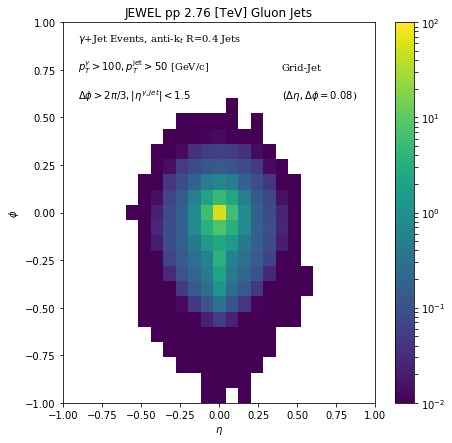
\includegraphics[width=0.45\textwidth]{plots/jewel_pp_avgGluonJet}
	   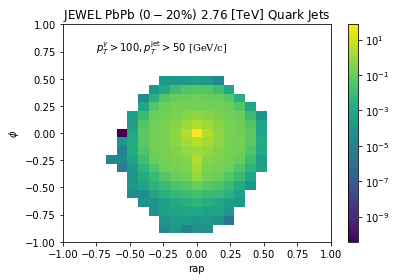
\includegraphics[width=0.45\textwidth]{plots/jewel_pbpb020_avgQuarkJet}
	   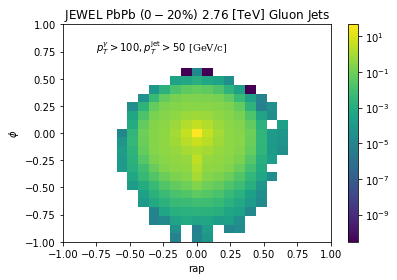
\includegraphics[width=0.45\textwidth]{plots/jewel_pbpb020_avgGluonJet}
	   \caption{Average quark (left) and gluon (right) pre-processed jet images shown in the $\eta-\phi$ plane for pp (top) and central PbPb (bottom) collisions generated from \jw. The color scale in the z axis represents the average pixel \pt in units of GeV/c. }
	   \label{fig:ave_jetimage_jewel}
	\end{figure}
	
	A deep convolutional neural network implemented in Keras with tensorflow backend is utilized in this analysis, motivated by recent studies in classifications of boosted objects in pp collisions~\cite{}. We have three 2-D convolution layers of sequentially reducing sizes each with 8 filters and followed by a corresponding max-pooling layer. Similar to our MVA analysis, each convolution layer  along with a hyperbolic tangent activation function. Each convolution layer is followed by a max-pooling layer and the final output has a sigmoid activation function. The output layer is preceded by a sequential a dropout layer with a rejection score of 0.20, dense layer with 20 nodes and an additional dropout layer with a reduced rejection score of 0.10. The additional dropout layer helps in filtering less important features from previous layers and thus increases the speed and efficiency of the classification model. The deep convolutional neural network model is trained with the Adam optimizer, with a binary cross entropy loss function, similar to our MVA model described above.
	
    %layer = Convolution2D(8, 11, 11, border_mode='same')(input_layer)
    %layer = Activation('tanh')(layer)
    %layer = MaxPooling2D(pool_size=(2,2))(layer)
    %layer = Convolution2D(8, 3, 3, border_mode='same')(layer)
    %layer = Activation('tanh')(layer)
    %layer = MaxPooling2D(pool_size=(3,3))(layer)
    %layer = Convolution2D(8, 3, 3, border_mode='same')(layer)
    %layer = Activation('tanh')(layer)
    %layer = MaxPooling2D(pool_size=(3,3))(layer)
    %layer = Flatten()(layer)
    %layer = Dropout(0.20)(layer)
    %layer = Dense(20)(layer)
    %layer = Dropout(0.10)(layer)
    %output_layer = Dense(1, activation='sigmoid', name='main_output')(layer)
    %model = Model(input=input_layer, output=output_layer)
    %model.compile(optimizer='adam', loss='binary_crossentropy', metrics=['accuracy'])


\subsection{Telescoping Deconstruction}
\label{sec:tjet}
	
In this section we apply telescoping deconstruction to quark/gluon discrimination \cite{Chien:2017decon} in both proton-proton and heavy ion collisions. It is a complete and systematic $N$-subjet expansion consisting simply of the subjet kinematic variables. The observables are combined using dense neural networks to maximize the tagging performance at each subjet order $N$. On the other hand, individual telescoping deconstruction observables are physically-meaningful which encode the all-order QCD splitting. We outline the procedure of the method and show how the subjet variables within this framework can reveal the full jet dynamics. In particular, we demonstrate the rich information of the subjet topology and subjet substructure contained at the T2 order, which is closely related to the groomed momentum sharing and the splitting function recently measured by the CMS collaboration. We also show how the subjet substructures allow us to extract the information about the partonic origins of the subjets. The quark/gluon tagging performances at each T$N$ order with increasing $N$ are shown to converge to the performance of the jet image technique using the convolutional neural network, and we compare the performances in proton-proton and heavy ion collisions. We see hints that the information contained in higher-order subleading subjets can be washed out in heavy ion collisions due to the huge underlying-event soft activities or, more interestingly, the thermal randomization caused by the medium interactions.

Telescoping deconstruction probes the radiation around dominant energy flows in a jet with multiple angular resolutions. It efficiently quantifies the radiation distribution by first capturing the dominant energy in the subjet reconstruction and then reaching out to include wide-angle, soft radiations. The procedure is outlined as below,
    \begin{itemize}
        \item At order $N$, determine $N$ axes $\{\hat n_i\}=\{(\eta_i,\phi_i)\}$ along the dominant energy flows, where $y$ and $\phi_i$ are the rapidity and the azimuthal angle of the subjet axis $i$. We use the $N$subjettiness 1-pass $k_T$ axes and the Winner-Take-All (WTA) $k_T$ axes \cite{Thaler:2010tr}.
        \item Construct $N$ subjets with $M$ radii $\{R_{T,m}\}^M_{m=1}$ by assigning particles to the nearest axis according to the distance $d^2_{ij} = \Delta y_{ij}^2+\Delta \phi_{ij}^2$ between the axis $\hat n_i$ and the particle $j$ \cite{Stewart:2010tn,Chien:2013kca,Stewart:2015waa,Thaler:2015xaa}.
            \begin{equation}
                {\rm subjet}_{i,m} = \{p^\mu_j~|~d_{ij}<R_{T,m}~{\rm and}~d_{ij}<d_{kj} \forall i\neq k\}.
            \end{equation}
            The subjet radii ${R_{T,m}}$ are sampled within the range $(0,R)$ where $R$ is the jet radius. In this paper $\{R_{T,m}\}$ are chosen to be evenly spaced within the range.
        \item We form the subjet data with the subjet transverse momenta and masses $\{(p_T,m)_{i,m}\}$,
            \begin{equation}
                {p_T}_{i,m}=\Big(\sum_{j\in~{\rm subjet}_{i,m}}p^\mu_j\Big)_T\;,~~~{m_{i,m}}^2=\Big(\sum_{j\in~{\rm subjet}_{i,m}}p^\mu_j\Big)^2\;,
            \end{equation}
            where we sum over all the particles $j$ within the subjet $i,m$. Together with the positions of the axes these form the telescoping deconstruction observables.
    \end{itemize}

We train a neural network on the subjet variables up to T$N$ order. The details about the neural network model can be found in \cite{Chien:2017decon}. We consider $N=\{1,2,3\}$ and the performance quickly saturates at $N=3$. Beside the overall quark/gluon tagging performance, we also examine the subjet variables at the T2 order representing the information of the subjet topology and the subjet substructure,
    \begin{equation}
        z=\frac{\min(p_{T_1},p_{T_2})}{p_{T_1}+p_{T_2}}\;,~~~~~m_l=\min(m_1,m_2)\;,~~~~~m_h=\max(m_1,m_2)\;,
    \end{equation}
where $z$ is the transverse-momentum fraction of the softer subjet and $m_{l(h)}$ is the light (heavy) subjet mass.

\section{Results}
\label{sec:results}

	% Add the final plots comparing the different methods
	
	List of plots to add
	
	1. ROC curve of just pp showing the MVA, DCNN and TD (telescoping deconstruction)

	2. ROC curve for pbpb same as above
	
	3. direct comparison of roc curve pp and PbPb MVA, DCNN and TC separate - 3 plots
	
	4. Comparing PbPb w/ and w/o grid and subtraction. talk about the effect on this.
	
    \begin{figure}
	   \centering
	   \includegraphics[width=0.45\textwidth]{plots/vacuum_medium_grid}
	   \includegraphics[width=0.45\textwidth]{plots/medium_grid_gridsub}
	   \caption{}
	   \label{fig:tjet}
	\end{figure}


\section{Conclusions}
\label{sec:conc}


\section*{Acknowledgments}
The authors would like to thank Benjamin Nachman and Sevil Salur for helpful discussions. This research was supported by the LHC Theory Initiative Postdoctoral Fellowship under the National Science Foundation grant PHY-1419008. RKE also acknowledges support from the National Science Foundation under Grant No.1067907 \& 1352081.

\appendix

Jets are collimated sprays of
particles observed at high energy colliders such as the Large Hadron Collider (LHC). Hard collisions produce energetic quarks and gluons, which shower and hadronize through the strong interaction into the final state particles captured by the detectors. This parton shower picture has been extremely successful for understanding and modeling jets. Physics at all energy scales enters %into
the parton shower and affects the final-state particle distribution. To extract specific features of the jet formation, many
%Many
physically motivated jet substructure observables, defined in terms of the observed particles, have been studied extensively \cite{Abdesselam:2010pt,Altheimer:2012mn,Altheimer:2013yza,Adams:2015hiv,Larkoski:2017jix,ATLAS-CONF-2017-064,Khachatryan:1955546}.

In this Letter, we go beyond \cite{Chien:2017xrb} and present the framework of telescoping deconstruction to systematically probe all aspects of jet formation. By scanning around dominant energy flows with multiple angular resolutions \cite{Chien:2013kca,Chien:2014hla}, one can efficiently quantify the radiation pattern. We demonstrate the use of the framework
in quark/gluon discrimination, boosted $W$ tagging and boosted top tagging, and we show that the framework captures all the relevant physics of jets. Crucially, the framework involves a fixed-order organization of individual observables which allows systematically improvable jet studies. Explicit examples of the $W$ isolation \cite{Chien:2017xrb} and exposing the $W$ boson in a top jet are presented. This highlights the physically meaningful nature of each telescoping deconstruction observables and demonstrates their collective power as a representation.

Recently, there has been progress in utilizing the complete information in a jet in an unbiased way %, typically making use of
using advanced machine-learning techniques. Powerful multivariate function approximators, such as neural networks, are capable of extracting useful features of the data relevant for a specific task. Examples include jet images with convolutional neural networks (CNNs)~\cite{Cogan:2014oua,deOliveira:2015xxd,Komiske:2016rsd,Kasieczka:2017nvn}, clustering histories with recurrent neural networks~\cite{Louppe:2017ipp}, and complete sets of high-level observables with dense neural networks (DNNs)~\cite{Datta:2017rhs,Datta:2017lxt,Aguilar-Saavedra:2017rzt}. See \cite{Larkoski:2017jix} for a more complete summary and discussion of recent progress. While machine-learning methods can provide large increases in performance, extracting physical messages from the trained neural network parameters is a complicated task.

Telescoping deconstruction aims to encapsulate all relevant physics information in very simple, physically-meaningful observables. The variables are close to the perturbative expansion of QCD and the parton shower picture therefore perturbative and nonperturbative physics information can be systematically extracted. Much like fixed-order perturbative expansions and parton shower splitting kernels \cite{Nagy:2017ggp}, the expansion is ordered by the number $N$ of exclusively reconstructed subjets. %axes.
At each order, %For a given order,
$N$ axes are determined by finding the dominant energy flow directions in the rapidity-azimuth plane~\cite{Stewart:2010tn,Chien:2013kca,Stewart:2015waa,Thaler:2015xaa}, which is partitioned into energy flow regions determined by the nearest axis. %Multiple
Jets at multiple angular resolutions are probed simply by the {\sl kinematics} of subjets consisting of %all
particles within different distances $R_T$ from %of
the energy flow axes.

\begin{figure*}[t]
\centering
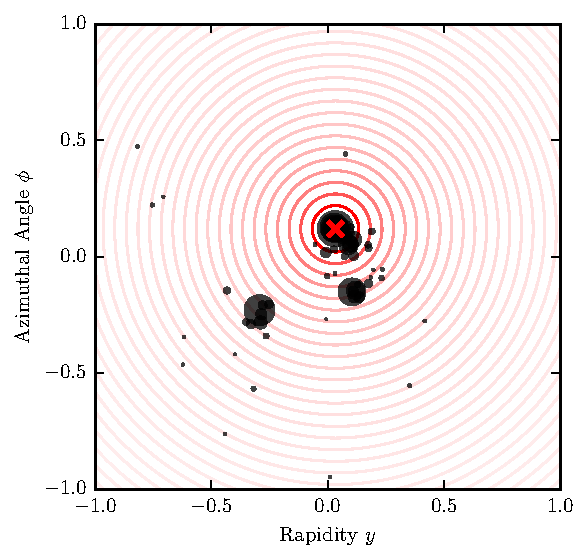
\includegraphics[width=.32\columnwidth]{figures/topjetT1_telescoped2.pdf}
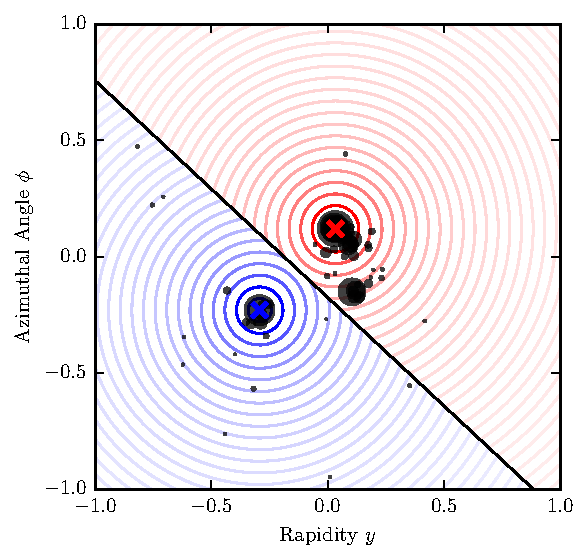
\includegraphics[width=.32\columnwidth]{figures/topjetT2_telescoped2.pdf}
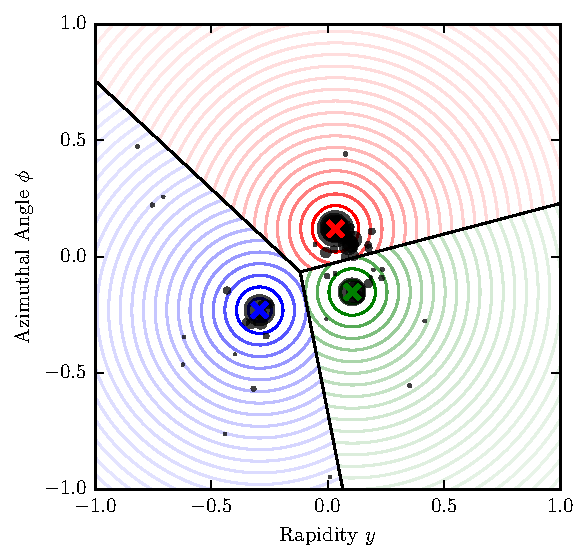
\includegraphics[width=.32\columnwidth]{figures/topjetT3_telescoped2.pdf}
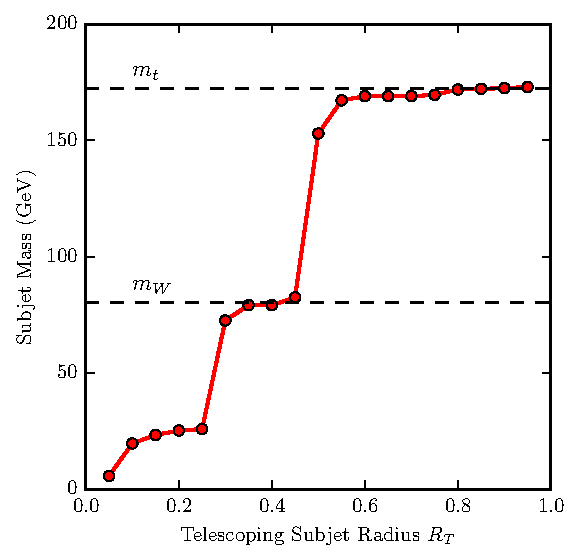
\includegraphics[width=.32\columnwidth]{figures/topjetT1_masses2.pdf}
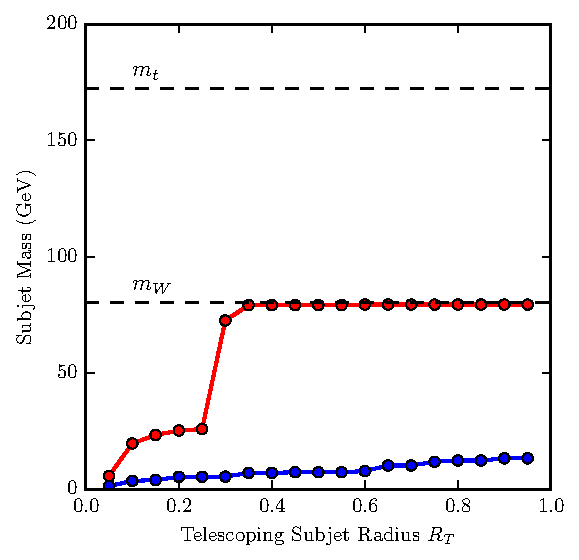
\includegraphics[width=.32\columnwidth]{figures/topjetT2_masses2.pdf}
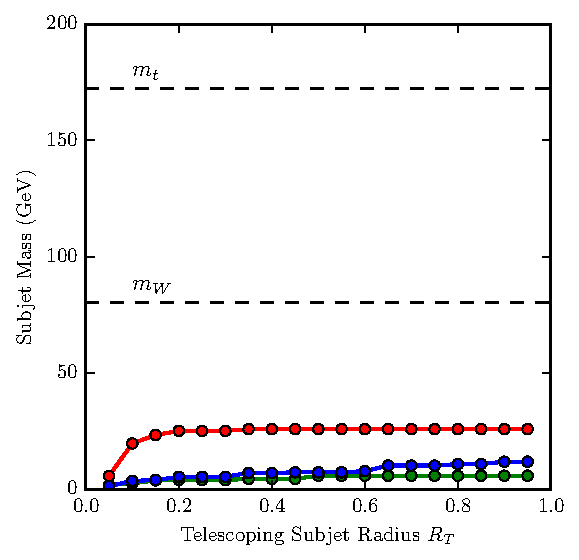
\includegraphics[width=.32\columnwidth]{figures/topjetT3_masses2.pdf}
\caption{\label{fig:tjet}(Top row) The telescoping deconstruction of a top jet at T1 (left panel), T2 (middle panel) and T3 (right panel) orders. The crosses are the Winner-Take-All $k_T$ axes. The straight lines are the exclusive subjet boundaries. Particles are sized according to their transverse momenta. (Bottom row) The subjet masses at T1 (left panel), T2 (middle panel), and T3 (right panel) orders as the telescoping radius $R_T$ is varied, corresponding to the region of the same color in the top row. The presence of the $W$ in the top jet can be clearly seen at T1 and T2 orders by the plateau of the red line beginning around $R_T=0.3$.}
\end{figure*}

The telescoping deconstruction procedure is: %substructure deconstruction is:
\begin{itemize}
        \item At order $N$, determine $N$ axes $\{\hat n_i\}=\{(\eta_i,\phi_i)\}$ along the dominant energy flows, where $y$ and $\phi_i$ are the rapidity and the azimuthal angle of the subjet axis $i$. We use the $N$subjettiness 1-pass $k_T$ axes and the Winner-Take-All (WTA) $k_T$ axes \cite{Thaler:2010tr}.
        \item Construct $N$ subjets with $M$ radii $\{R_{T,m}\}^M_{m=1}$ by assigning particles to the nearest axis according to the distance $d^2_{ij} = \Delta y_{ij}^2+\Delta \phi_{ij}^2$ between the axis $\hat n_i$ and the particle $j$ \cite{Stewart:2010tn,Chien:2013kca,Stewart:2015waa,Thaler:2015xaa}.
            \begin{equation}
                {\rm subjet}_{i,m} = \{p^\mu_j~|~d_{ij}<R_{T,m}~{\rm and}~d_{ij}<d_{kj} \forall i\neq k\}.
            \end{equation}
            The subjet radii ${R_{T,m}}$ are sampled within the range $(0,R)$ where $R$ is the jet radius. In this paper $\{R_{T,m}\}$ are chosen to be evenly spaced within the range.
        \item We form the subjet data with the subjet transverse momenta and masses $\{(p_T,m)_{i,m}\}$,
            \begin{equation}
                {p_T}_{i,m}=\Big(\sum_{j\in~{\rm subjet}_{i,m}}p^\mu_j\Big)_T\;,~~~{m_{i,m}}^2=\Big(\sum_{j\in~{\rm subjet}_{i,m}}p^\mu_j\Big)^2\;,
            \end{equation}
            where we sum over all the particles $j$ within the subjet $i,m$. Together with the positions of the axes these form the telescoping deconstruction observables.
    \end{itemize}

The telescoping deconstruction observables fall into two categories~\cite{Chien:2017xrb}: the {\sl subjet topology}, which is described by the axes and subjet transverse momenta, and the {\sl subjet substructure}, quantified by the subjet masses. {\sl Subjet charge}~\cite{Krohn:2012fg} information can straightforwardly be included in this framework as well. As the telescoping subjet order $N$ (T$N$ order) increases, more jet energy is covered by the subjets and the number of subjet radii sampled can be systematically decreased. In the large $N$ limit, the subjets reduce to individual particles %and
thus the basis is formally shown to be complete. The telescoping deconstruction allows one to easily exploit features both within each subjet and among all the subjets. See \Fig{fig:tjet} for the telescoping deconstruction of a top jet for $N = 1$, $2$, and $3$ where the $W$ resonance can clearly be seen.

To demonstrate the efficacy of telescoping deconstruction in capturing the full jet information,
we demonstrate the framework in quark/gluon discrimination, boosted $W$ tagging and boosted top tagging. Each of these problems have
signal jets with a different characteristic number of prongs: one, two, and three prongs, respectively. Events were generated from Monte Carlo simulation of proton-proton collisions at 14 TeV using \textsc{Pythia} 8.226~\cite{Sjostrand:2007gs}. Final-state non-neutrino particles are clustered into jets with \textsc{FastJet} 3.3.0~\cite{Cacciari:2011ma} using the anti-$k_T$ algorithm~\cite{Cacciari:2008gp}. We consider the boosted regime with the jet $p_T$ between 800 GeV and 900 GeV. For quark/gluon discrimination, quark jets were generated by $pp\to q+Z(\to\nu\bar\nu)$ and gluon jets %were generated
by $pp\to g + Z(\to\nu\bar\nu)$, clustered into $R=0.4$ jets with rapidity $|y|<1.5$.

\begin{figure*}[t]
\centering
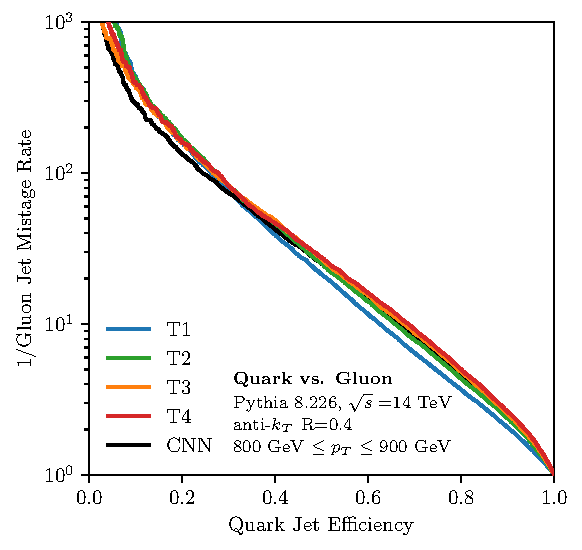
\includegraphics[width=.32\columnwidth]{figures/QG_invROC.pdf} 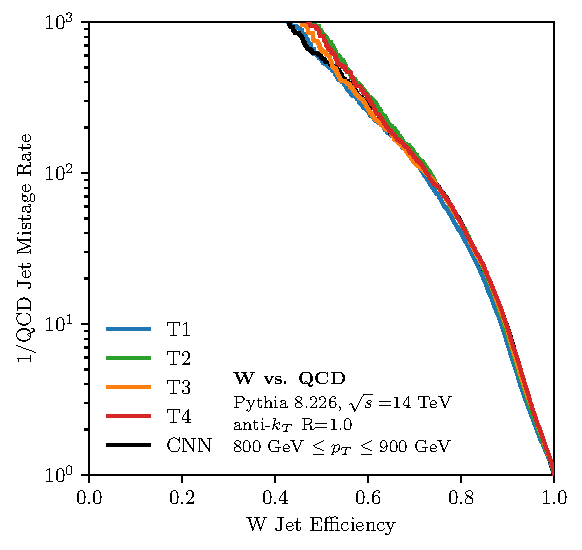
\includegraphics[width=.32\columnwidth]{figures/W_invROC.pdf} 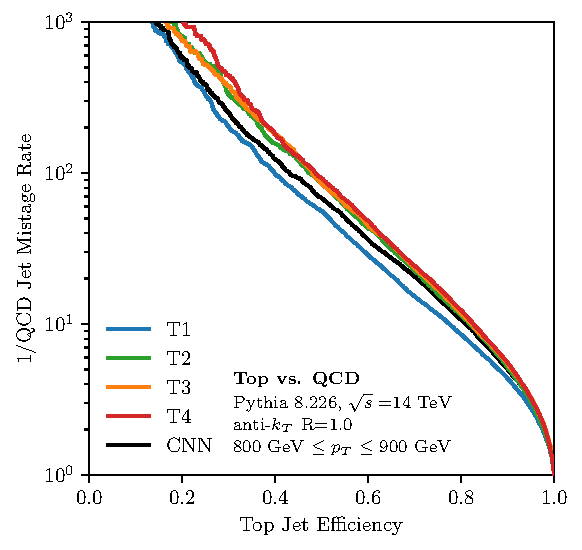
\includegraphics[width=.32\columnwidth]{figures/Top_invROC.pdf}
\caption{\label{ROCs}ROC curves for the DNNs trained on cumulant telescoping deconstruction observables up to T1 through T4 orders and the jet image method using CNNs for quark/gluon discrimination (left panel), boosted $W$ (middle panel) and top (right panel) tagging. The T$N$ performance approximately saturates at T2 (quark/gluon), T1 ($W$ tagging), and T2 (top tagging) orders.}
\end{figure*}

Since $W$ and top tagging are mass resonance searches where the jet mass is the most natural and powerful discriminating variable, we disentangle mass information to probe how much additional information can be exploited for tagging. Information from the hard process about the overall jet kinematics is eliminated by translating each jet to a frame where $y$ and $\phi$ of the jet are both zero. For $W$ and top tagging, $W$ jets were generated by $pp\to WW (\to \text{hadrons})$ and top jets were generated by $pp\to t\bar t (\to \text{hadrons})$, with background jets from QCD dijets. Final-state non-neutrino particles are clustered into $R=1.0$ jets with rapidity $|y|<1.5$. Signal and background jets identically populate a five-bin $1/p_T^4$ histogram in transverse momentum and a three-bin uniform histogram in mass between 75 GeV and 85 GeV for $W$ tagging and 160 GeV to 180 GeV for top tagging. Telescoping subjets are constructed with $R_T$ in steps of 0.05 between 0.05 and 0.4 in
quark/gluon discrimination, and between 0.05 to 0.95 in
$W$ and top tagging. Reducing the number of radius sampling is left for future work. For each problem, 200k events are generated for signal and background, with 10\% used for validation, 15\% for testing, and the remaining 75\% for training.

A neural network consisting of three dense layers with 100 nodes each is trained on the telescoping deconstruction observables up to T$N$ order. The training can be performed on a typical laptop CPU in fewer than five minutes. One could also use boosted decision trees to combine variables \cite{Chien:2017xrb}. We compare the performance of our method to jet images using a CNN, which requires a graphics processing unit (GPU) to train. The jet images are size $33\times 33$ and span a $2R\times 2R$ patch of the rapidity-azimuth plane with the intensity of each pixel corresponding to the total $p_T$ of particles in the pixel. The jet images are standardized according to the procedure in \Ref{Komiske:2016rsd}. The CNN architecture consists of three 48-filter convolutional layers with filter sizes of $8\times 8$, $4\times 4$, and $4\times 4$ followed by a 128-unit dense layer and a 2-unit softmaxed output layer. A $2\times 2$ maxpooling is performed after each convolutional layer with a stride length of 2. The dropout rate was taken to be 0.1 for all layers. All neural networks are implemented using the Python deep learning library Keras~\cite{keras} with the Theano backend~\cite{bergstra2010theano}. Rectified linear unit (ReLU) activation functions~\cite{nair2010rectified} and He-uniform model weight initialization~\cite{heuniform} are used. The networks are trained using the Adam algorithm~\cite{adam} with a learning rate of $10^{-3}$ and a batch size of 256 for 50 epochs with a patience parameter of 8, and the best model is selected based on validation set performance.

The performance of the trained models can be captured in a Receiver Operating Characteristic (ROC) curve which plots the inverse of the background mistag rate at different signal efficiencies, where a higher curve indicates better classification performance. \Fig{ROCs} shows the ROC curves for the three tagging problems of the models trained on the cumulant telescoping deconstruction observables up to T$N$ order for $N\in\{1,2,3,4\}$ and the CNNs trained on jet images. The T$N$ performance converges quickly and is comparable to the performance of the jet images approach. % Note that since
The CNN architecture has not been tuned exhaustively, therefore its ROC curves serve to give a general sense of performance. %This is highlighted in the top case, where the telescoping deconstruction DNN outperforms the CNN at T2 order and above.
\begin{figure*}
\centering
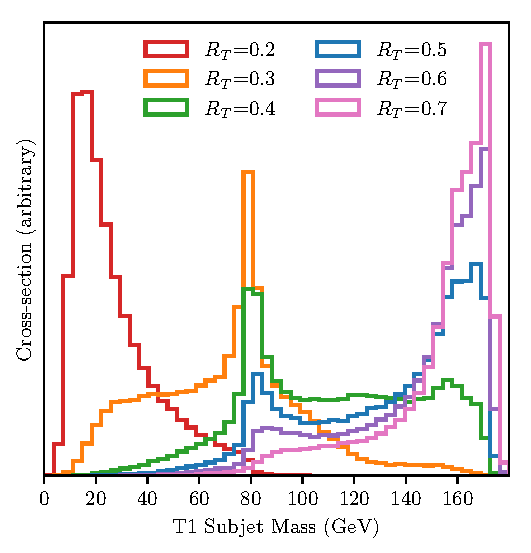
\includegraphics[width=.32\columnwidth]{figures/T1HeavyMass_top.pdf}
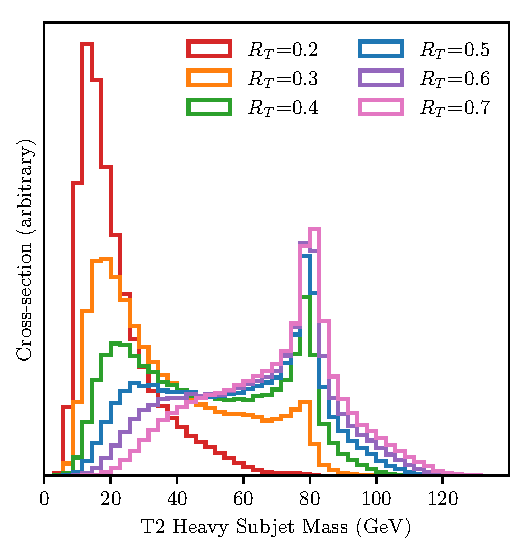
\includegraphics[width=.32\columnwidth]{figures/T2HeavyMass_top.pdf}
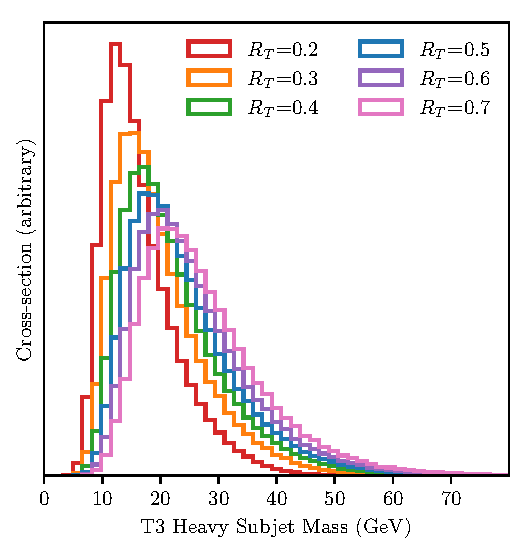
\includegraphics[width=.32\columnwidth]{figures/T3HeavyMass_top.pdf}
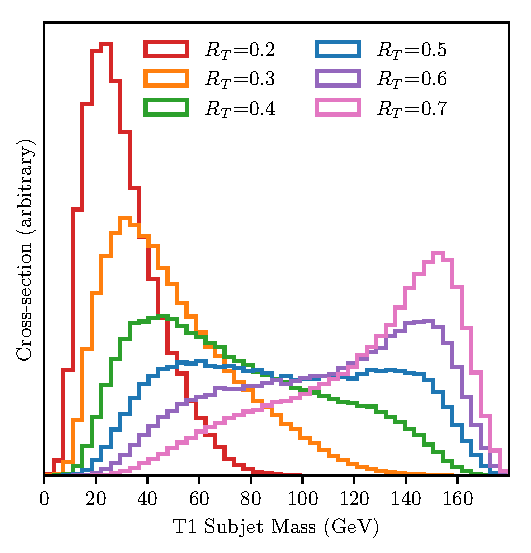
\includegraphics[width=.32\columnwidth]{figures/T1HeavyMass_qcd.pdf}
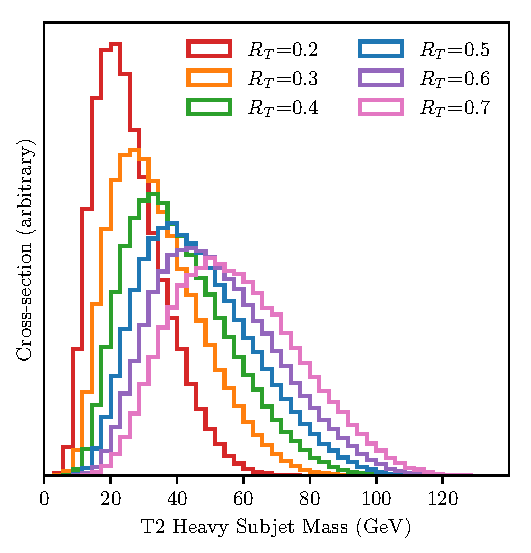
\includegraphics[width=.32\columnwidth]{figures/T2HeavyMass_qcd.pdf}
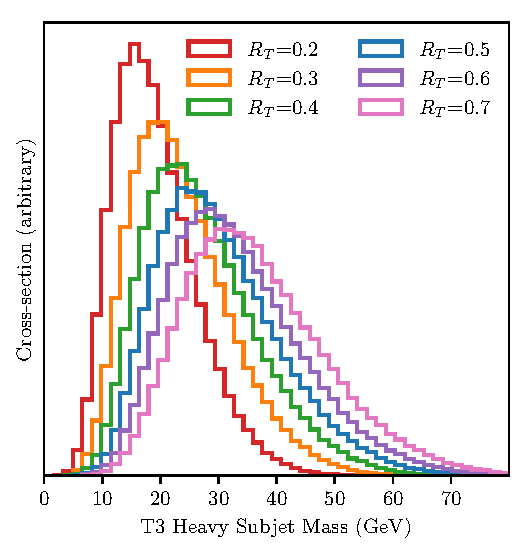
\includegraphics[width=.32\columnwidth]{figures/T3HeavyMass_qcd.pdf}
\caption{\label{masses}The heavy subjet mass distributions at T1 (left panels), T2 (middle panels), and T3 (right panels) orders for multiple subjet radii $R_T$ of top jets (top row) and QCD background jets (bottom row). The presence of the $W$ in top jets is evident by the peaks at the $W$ mass at T1 and T2 orders. At T3 order, the heavy subjet mass distributions are QCD-like and are narrower (more quark-like) in %the case of
top subjets than the wider (more gluon-like) QCD subjets. These features highlight the ability of the telescoping deconstruction to probe subjet substructure.}
\end{figure*}

For top tagging, there is a significant increase in performance from T1 to T2 order in \Fig{ROCs}, and the performance saturates beyond this order due to the sensitivity of T2 to the $W$ in top jets. For $W$ tagging, T1 order is sufficient to achieve most of the classification performance, which unambiguously confirms the $W$ isolation feature in the boosted regime compared to the QCD background~\cite{Chien:2017xrb}. Clearly, the T1 order probes the depletion of the radiation at large angles within $W$ jets, whereas the QCD background jets continue to accrue mass from radiation at large angles. For quark/gluon discrimination, there is a significant increase in performance from T1 to T2 and a smaller increase from T2 to T3 where the performance saturates, suggesting the usefulness of T2 subjet substructure and its sensitivity to subjet flavors. This confirms that the T$N$ expansion converges efficiently and telescoping deconstruction faithfully represents the jet information.

In addition to being a complete jet representation, the telescoping deconstruction allows physical information to be easily extracted. \Fig{masses} shows the heavy subjet mass distributions at T1, T2, and T3 orders, scanned over different telescoping radii $R_T$, for top jets and their QCD background. As $R_T$ is increased, the top jet T1 subjet mass distributions transition from QCD-like, to peaked at the $W$ mass, to peaked at the top mass. In contrast, the background QCD jets do not peak at the $W$ mass for any $R_T$ and transition from QCD-like to more top-like as they %continue to
accrue mass at larger radii. The top jets at T2 order clearly and automatically show the $W$ peak which is completely absent in the background distributions. At T3 order, both top and background distributions appear QCD-like, with the wider background distributions %slightly wider
due to the prevalence of gluon subjets. This highlights again subjet substructure in telescoping deconstruction.

To conclude, we present the telescoping deconstruction framework as a complete, physically-motivated expansion of the jet.
%Neural networks were trained on the telescoping deconstruction observables up to different T$N$ orders and applied to quark/gluon discrimination, boosted $W$ and top tagging.
Telescoping deconstruction observables up to different T$N$ orders are combined using multivariate methods and applied to quark/gluon discrimination, boosted $W$ and top tagging.
%The performance of the models indicates that the
The T$N$ performance converges efficiently and compares favorably to a CNN trained on jet images. Further, the individual telescoping deconstruction observables were shown to cleanly encode relevant features of jets such as the isolation of $W$ jets, the presence of the $W$ in top jets, and the quark- or gluon- like nature of the heaviest prongs in top and QCD jets. This complete and general framework is suitable for systematic studies of full jet dynamics, with rich future applications in parton-shower tuning, heavy ion hard probe studies \cite{Chien:2017hij}, and identification of hadronic electroweak-boson emissions in ultra-high energy jets. The extension to hard-process tagging and resonance search at the event level is also promising.



\bibliographystyle{JHEP3}
\bibliography{qg_ML_ref}

\end{document}

































































